% \iffalse
\let\negmedspace\undefined
\let\negthickspace\undefined
\documentclass[journal,12pt,twocolumn]{IEEEtran}
\usepackage{cite}
\usepackage{amsmath,amssymb,amsfonts,amsthm}
\usepackage{algorithmic}
\usepackage{graphicx}
\usepackage{textcomp}
\usepackage{xcolor}
\usepackage{txfonts}
\usepackage{listings}
\usepackage{enumitem}
\usepackage{mathtools}
\usepackage{gensymb}
\usepackage{comment}
\usepackage[breaklinks=true]{hyperref}
\usepackage{tkz-euclide} 
\usepackage{listings}
\usepackage{gvv}                                        
\def\inputGnumericTable{}                                 
\usepackage[latin1]{inputenc}                                
\usepackage{color}                                            
\usepackage{array}                                            
\usepackage{longtable}                                       
\usepackage{calc}                                             
\usepackage{multirow}                                         
\usepackage{hhline}                                           
\usepackage{ifthen}                                           
\usepackage{lscape}
\usepackage[export]{adjustbox}

\newtheorem{theorem}{Theorem}[section]
\newtheorem{problem}{Problem}
\newtheorem{proposition}{Proposition}[section]
\newtheorem{lemma}{Lemma}[section]
\newtheorem{corollary}[theorem]{Corollary}
\newtheorem{example}{Example}[section]
\newtheorem{definition}[problem]{Definition}
\newcommand{\BEQA}{\begin{eqnarray}}
\newcommand{\EEQA}{\end{eqnarray}}
\newcommand{\define}{\stackrel{\triangle}{=}}
\theoremstyle{remark}
\newtheorem{rem}{Remark}
\begin{document}
\parindent 0px
\bibliographystyle{IEEEtran}
\vspace{3cm}

\title{Assignment\\[1ex]12.8 - 6}
\author{EE23BTECH11034 - Prabhat Kukunuri$^{}$% <-this % stops a space
}
\maketitle
\newpage
\bigskip

\renewcommand{\thefigure}{\theenumi}
\renewcommand{\thetable}{\theenumi}
\section*{Question}
A charged particle oscillates about its mean equilibrium position with a frequency of $10^9$ Hz. What is the frequency of the electromagnetic waves produced by the oscillator?

\section*{Solution}
An oscillating charged particle in space produces electromagnetic waves. The frequency of the generated electromagnetic waves is equal to the frequency of the oscillating charged particle.
\begin{align}
    f = f_{osc}
\end{align}
The oscillating frequency of charged particle is $10^9$
\begin{align}
    f = 10^9
\end{align}
The frequency of the electromagnetic waves produced by the oscillator is $10^9$ Hz.
\vspace{0.2in}

The equation for amplitude of electromagnetic wave is of the form 
\begin{align}
    y = \cos\left({\dfrac{2}{\pi}\nu t}\right)
\end{align}
\hspace{0.25in}
$\nu$ is the frequency of the electromagnetic wave.

\hspace{0.25in}
$y$ is the amplitude of the electromagnetic wave.
\vspace{0.2in}

For the electro-magnetic wave generated due to oscillation charged particle amplitude is related to time by
\begin{align}
    y = \cos\left({\dfrac{2}{\pi}\times 10^9 t}\right)
\end{align}
\vspace{0.2in}

Plotting the amplitude of the electromagnetic wave as a function of time
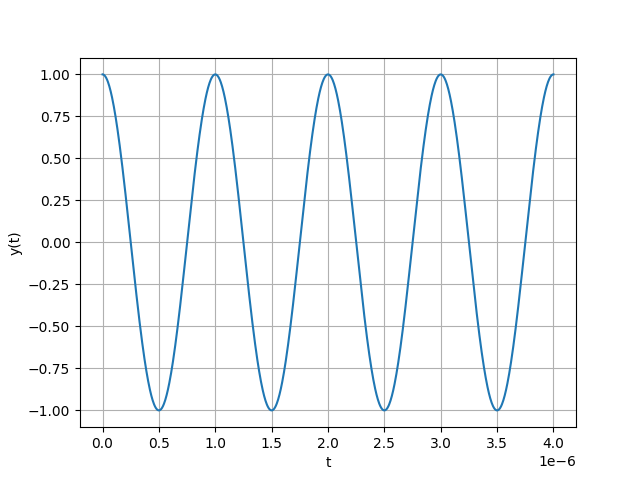
\includegraphics[width=4in,height=3in]{Figure_1.png}
\end{document}
